\documentclass{article}
\usepackage{graphicx}
\begin{document}
PA $2$ :\\
1. The coefficients for the natural cubic spline :\\
\begin{tabular}{c|c|c|c|c|c}
$i$&$x_i$&$a_i$&$b_i$&$c_i$&$d_i$\\
\hline
0&0.9&1.3&0.5396238492562306&0.0&-0.2476490578514421\\
1&1.3&1.5&0.4207523014875384&-0.29717886942173055&0.9469120930523156\\
2&1.9&1.85&1.086802718677962&1.407262898072437&-2.956382457311267\\
3&2.1&2.1&1.294941983029585&-0.36656657631432493&-0.44663477948968966\\
4&2.6&2.6&0.5933993220979927&-1.0365187455488594&0.44505110075969534\\
5&3.0&2.7&-0.022191145976440896&-0.5024574246372251&0.17415987014396273\\
6&3.9&2.4&-0.5034060258736166&-0.032225775248525754&0.07807565399151953\\
7&4.4&2.15&-0.4770750606285027&0.08488770573875365&1.314171284150477\\
8&4.7&2.05&-0.07131619046462218&1.267641861474182&-1.5812189034551638\\
9&5.0&2.1&0.2623398224869929&-0.15545515163546453&0.04311532914847155\\
10&6.0&2.25&0.08077550666147848&-0.026109164190049883&-0.004666342471428775\\
11&7.0&2.3&0.01455815086709239&-0.04010819160433621&-0.024449959262756\\
12&8.0&2.25&-0.13900811012984798&-0.11345806939260421&0.017470689861786695\\
13&9.2&1.95&-0.33583409646917955&-0.05056358589017213&-0.012727908254745292\\
14&10.5&1.4&-0.5318299146351858&-0.1002024280836788&-0.02032522327792245\\
15&11.3&0.9&-0.7311782282626832&-0.14898296395069272&1.213405008680248\\
16&11.6&0.7&-0.4929486542894339&0.9430815438615265&-0.8392747703448531\\
17&12.0&0.6&-0.14133530896574226&-0.06404818055229802&0.03638208508459536\\
18&12.6&0.5&-0.17890047373713686&0.0014395725999735848&-0.4479709706428262\\
19&13.0&0.4&-0.392774881565715&-0.5361255921714183&0.5956951024126856\\
\end{tabular} \\
\\
\\
2. The coefficients for the interpolating polynomial :\\
\begin{tabular}{c|c}
i&$F_{i,i}$\\
\hline
1&0.4999999999999999\\
2&0.08333333333333372\\
3&0.6249999999999981\\
4&-0.9063240680887712\\
5&0.5668351256586526\\
6&-0.18391194861782978\\
7&0.03874690604922625\\
8&-0.0025481504155956077\\
9&-0.0018586750299486596\\
10&0.0005729317636593806\\
11&-6.34107592999165e-06\\
12&-4.290233994816249e-05\\
13&1.5798171679188234e-05\\
14&-3.453534469332749e-06\\
15&6.085950046764253e-07\\
16&-9.860361084436146e-08\\
17&1.4695484208907752e-08\\
18&-1.9837133192976805e-09\\
19&2.5185394950467503e-10\\
20&-3.0745307801080036e-11\\
\end{tabular}\\
\\
3. The graph in problem 3 :\\
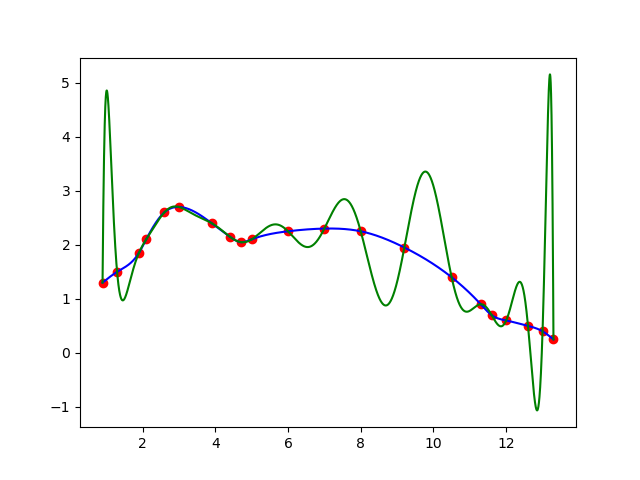
\includegraphics[scale=0.6]{1.png}\\
The red points are the points of the given datas.\\
The blue line is the plot of the cubic spline.\\
The green line is the plot of the interpolating polynomial.\\
\end{document}
